\documentclass{beamer}
\usetheme{Frankfurt}

\usepackage{listings}

\newcommand{\todo}[1]{\alert{TODO #1}}

\title{Introduction}
\subtitle{Lecture 1 \\ Computer Security DD2395}
\author[R. Guanciale]{
  Roberto Guanciale\\
  robertog@kth.se
}
\date{2013-10-03}
\begin{document}

\begin{frame}[plain]
  \titlepage
\end{frame}

\begin{frame}{Outline for Today}
  \begin{itemize}
    \item About me
    \item About the course
    \item About you
    \item About computer security
  \end{itemize}
\end{frame}

\begin{frame}{About Roberto Guanciale}
  \begin{itemize}
    \item PostDoc on formal verification
    \item Enthusiast software developer
    \item robertog@kth.se
    \item \alert{Always} use the e-mail subject: [DD2395] ...
    \item Office: \todo{level 5, room 4424}
    \item You are welcomed (no booking required, no fee) Wednesday:
      14:00-15:00
  \end{itemize}
\end{frame}

\begin{frame}{About the course}
  Lectures and Labs
  \begin{itemize}
    \item From now until December
    \item Ca. 3 ECTS in P1 and 3 ECTS in P2
    \item Labs start \todo{September 18}
  \end{itemize}
\end{frame}

\begin{frame}{General Goals}
  \begin{itemize}
    \item Learn about security concepts
    \item Have tools and methods to reason about security
    \item Spot threats, vulnerabilities
    \item Know, propose and evaluate counter-measures
    \item Present concepts to others 
  \end{itemize}
\end{frame}

\begin{frame}{Learning Outcomes}
  You should be able to
  \begin{itemize}
    \item recognize threats to confidentiality, integrity, and
      availability of systems
    \item explain the basic computer security terminology and concepts
      and use them correctly 
    \item find and apply documentation of security-related problems
      and tools 
    \item analyze code or system descriptions in terms
      of their security
    \item identify vulnerabilities of such code or descriptions and
      predict their corresponding threats
    \item compare counter-measures and evaluate their side-effects
    \item present and explain your reasoning to others
  \end{itemize}
\end{frame}

\begin{frame}{People}
  \begin{itemize}
    \item Course leader/exams: Roberto Guanciale
    \item Former Course leader/exams: Sonja Buchegger (KTH professor)
    \item Invited speakers:
      Alexander Baltatzis,
      Olof Hagsand,
      Gunnar Karlsson,
      Mikael,
      OWASP,
      Marten Trolin 
    \item Lab assistants: 
      Benjamin Greschbach,
      Guillermo Rodriguez Cano
  \end{itemize}
\end{frame}

\begin{frame}{Course info and breaking news}
  \begin{itemize}
    \item Check course website regularly for updates!
    \item DD2395 dasak13 on KTH Social
    \item https://www.kth.se/social/course/DD2395/
  \end{itemize}
\end{frame}

\begin{frame}{Times and Places}
  \begin{itemize}
    \item look at schema, course code DD2395
  \end{itemize}
\end{frame}

\begin{frame}{Lectures Content}
  \begin{tabular}{cl|cl}
    01 & Admin, Intro [Ch.1] &
    02 & Operating systems \\
    03 & Computer networking &
    04 & Cryptography [2,20] \\
    05 & Authentication [3] &
    06 & Web security \\
    07 & Access control [4] &
    08 & Intrusion detection [8] \\
    09 & Firewalls [9] &
    10 & Malware [7] \\
    11 & Denial of Service [8] &
    12 & Multi-level security [10] \\
    13 & Audits &
    14 & Buffer overflows [11] \\
    15 & Software engineering &
    16 & Social engineering
  \end{tabular}
\end{frame}

\begin{frame}{Lab Exercises}
  \begin{itemize}
    \item See schema for times and rooms
    \item Instructions on web site on \todo{September 11}
    \item 4 different exercises
      \begin{enumerate}
        \item on GnuPG, remote or at CSC
        \item on iptables/firewalls, at CSC
        \item on web attacks, remote or at CSC
        \item presentation at CSC, report, assess
      \end{enumerate}
  \end{itemize}
\end{frame}

\begin{frame}{Seminar}
  \begin{itemize}
    \item Presentation and demo on computer security 
      topic in a seminar
    \item Groups of 2-3 students
    \item Topics will be published on the website
    \item Group seminars, schedule in schema, 
      signup on course website
  \end{itemize}
\end{frame}

\begin{frame}{Deadlines}
  \todo{Fridays, at 5pm}
  \begin{itemize}
  \item 28/9 GPG lab completion 
  \item 5/10 Iptables lab registration 
  \item 12/10 Seminar topic registration 
  \item 26/10 Web attacks lab completion 
  \item 2/11 Seminar time registration 
  \item 9/11 Seminar report completion 
  \item 16/11 Seminar feedback completion 
  \end{itemize}
\end{frame}

\begin{frame}{Exam}
  \begin{itemize}
  \item \todo{December 14, 2013}
  \item \alert{Mandatory} registration 
  \item \todo{Re-exam in June 2014}
  \end{itemize}
\end{frame}

\begin{frame}{Assessment, Grades}
  \begin{itemize}
  \item 6 ECTS in total, $\sim$ 160 hours of work 
  \item 3 ECTS Exam $\in [A \dots F]$
  \item 3 ECTS Labs $\in \{pass,fail\}$, no grades
  \item bonus points for exam (once) when bonus 
    requirements of lab fulfilled, see lab descriptions
  \end{itemize}
\end{frame}

\begin{frame}{Main didactic material}
  \begin{itemize}
  \item William Stallings and Lawrie Brown, Computer Security:
    Principles and Practice, published by Pearson 
  \item Ross Anderson, Security Engineering, Free online
  \item \todo{images}
  \end{itemize}
\end{frame}

\begin{frame}{Language}
  \begin{itemize}
  \item Lectures and texts in English
  \item OS lecture in Swedish
  \item Mails/website/etc in English
  \end{itemize}
\end{frame}

\begin{frame}{Accounts}
  \begin{itemize}
  \item Needed for lab exercises
  \item Who doesn't have an account and access card?
  \item Go to the systems group counter, Delfi, entry 
floor of Osquars Backe 2
  \end{itemize}
\end{frame}

\begin{frame}{RAPP}
  \begin{itemize}
    \item Register for DD2395, if not already done so 
    \item Specify that you're taking the course 
    \item \todo{https://rapp.csc.kth.se/rapp/}
  \end{itemize}
\end{frame}
 
\begin{frame}{Course Responsible Students }
  \begin{itemize}
  \item Select 2 students amongst yourselves 
  \item Introduce yourselves to me at a lecture 
  \end{itemize}
\end{frame}


\begin{frame}{Next Courses}
  \begin{itemize}
  \item Networking Security with Johan Karlander
  \item Foundations of Cryptography with Douglas Wikstr\:om
  \item Software Security with Dilian Gurov
  \item Networking Security courses with Panos
    Papadimitratos at EES
  \end{itemize}
\end{frame}

\begin{frame}{Honor}
  \begin{itemize}
  \item CSC Honor code +
  \item \alert{Do not attack a running system 
    without the consent of the owner 
    and the users}
  \item Defense Against the Dark Arts
  \end{itemize}
  \center{
  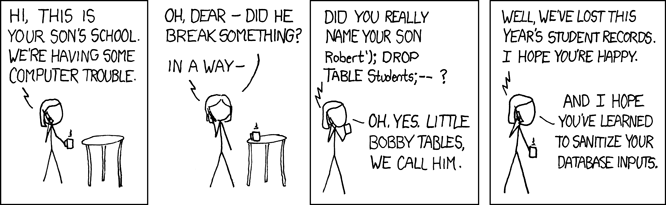
\includegraphics[width=0.7\linewidth]{exploits_of_a_mom}
  }
\end{frame}

\begin{frame}{Questions}
  \begin{itemize}
  \item ?????????????????????????
  \end{itemize}
\end{frame}

\begin{frame}{Computer Security}
  \begin{itemize}
  \item Computer Security: Principles and Practice
  \item by William Stallings and Lawrie Brown
  \end{itemize}
\end{frame}

\begin{frame}{Overview}
  \begin{itemize}
  \item \alert{Computer Security}: protection afforded to an 
    automated information system in order to attain 
    the applicable objectives of preserving
    
    \begin{itemize}
    \item integrity
    \item availability
    \item confidentiality
    \end{itemize}
of  information system resources, including
 
\begin{itemize}
  \item hardware
  \item software
  \item firmware
  \item information/data
  \item telecommunications
\end{itemize}
  \end{itemize}
\end{frame}

\begin{frame}{Key Security Concepts}
  \begin{center}
    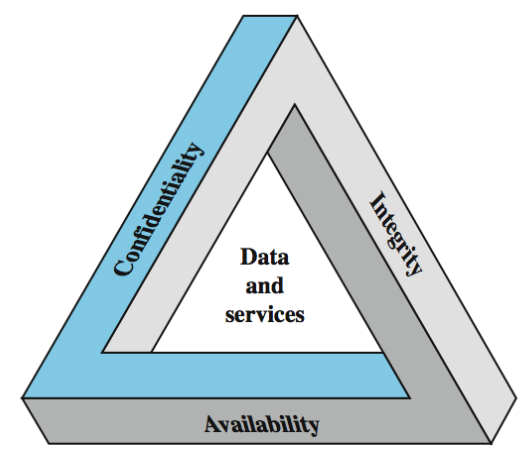
\includegraphics[width=0.7\linewidth]{concepts}
  \end{center}
\end{frame}

\begin{frame}{Levels of impact}
  \begin{itemize}
  \item Low
    \begin{itemize}
      \item Confidentiality of student list
      \item Integrity of on-line pools
      \item Availability of a node in peer-to-peer file sharing
    \end{itemize}
  \item Moderate    
    \begin{itemize}
      \item Confidentiality of student grade
      \item Integrity of a web forum
    \end{itemize}
  \item High
    \begin{itemize}
      \item Availability of SCADA systems
      \item Integrity of financial transactions
    \end{itemize}
  \end{itemize}
\end{frame}

\begin{frame}{Challenges}
  \begin{itemize}
  \item Security can be hard to achieve. Why? 
  \item Think about it for 2 min. 
  \item Turn to your neighbor and discuss for 3 min.
  \end{itemize}
\end{frame}
 
\begin{frame}{Computer Security Challenges}
  \begin{itemize}
\item not simple in complex systems 
\item must consider potential attacks 
\item procedures used counter-intuitive 
\item involve algorithms and secret info 
\item must decide where to deploy mechanisms 
\item battle of wits between attacker / admin 
\item not perceived on benefit until fails 
\item requires regular monitoring 
\item too often an after-thought 
\item regarded as impediment to using system
  \end{itemize}
\end{frame}


\begin{frame}{Security Terminology}
  \begin{center}
    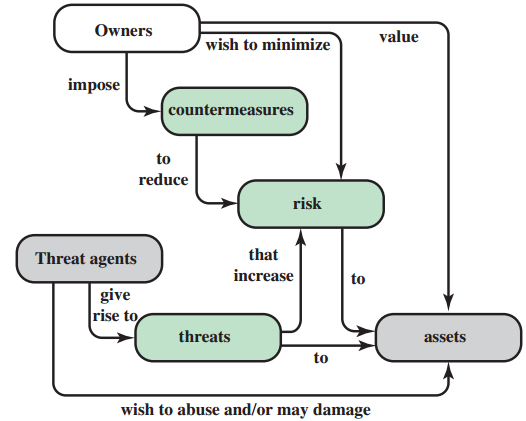
\includegraphics[width=0.7\linewidth]{terminology}
  \end{center}
\end{frame}

\begin{frame}{Security Terminology}
  \begin{center}
    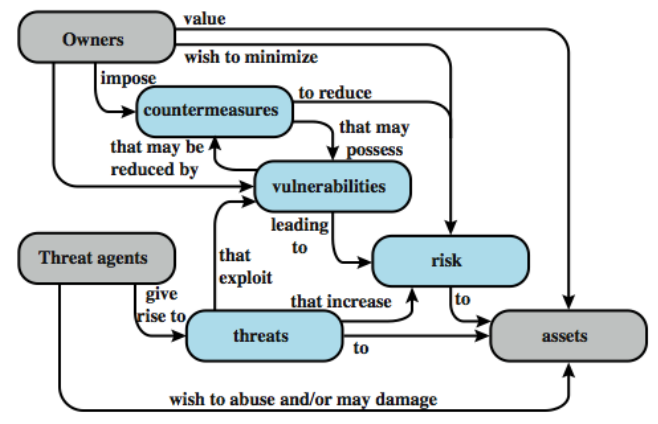
\includegraphics[width=0.7\linewidth]{terminology2}
  \end{center}
\end{frame}

\begin{frame}{Vulnerabilities and Attacks }
  \begin{itemize}
    \item system resource vulnerabilities may 
      
      \begin{itemize}
        \item be corrupted (loss of integrity) 
        \item become leaky (loss of confidentiality) 
        \item become unavailable (loss of availability) 
      \end{itemize}
    \item attacks are threats carried out and may be 
      \begin{itemize}
        \item passive
        \item active
        \item insider
        \item outsider
      \end{itemize}
  \end{itemize}
\end{frame}

\begin{frame}{Countermeasures}
  
  \begin{itemize}
    \item means used to deal with security attacks 
      
      \begin{itemize}
        \item prevent 
        \item detect 
        \item recover 
      \end{itemize}
    \item may result in new vulnerabilities 
    \item will have residual vulnerability 
    \item goal is to minimize risk given constraints
  \end{itemize}
\end{frame}


\begin{frame}{Threat Consequences}
  \begin{itemize}
    \item unauthorized disclosure 
      \begin{itemize}
        \item exposure, interception, inference, intrusion 
        \end{itemize}
      \end{itemize}
  \begin{itemize}
    \item deception 
      \begin{itemize}
        \item masquerade, falsification, repudiation 
        \end{itemize}
      \end{itemize}
  \begin{itemize}
    \item disruption 
      \begin{itemize}
        \item incapacitation, corruption, obstruction 
        \end{itemize}
      \end{itemize}
  \begin{itemize}
    \item usurpation 
      \begin{itemize}
      \item misappropriation, misuse
      \end{itemize}
    \end{itemize}
\end{frame}

\begin{frame}{Scope of Computer Security}
  \begin{center}
    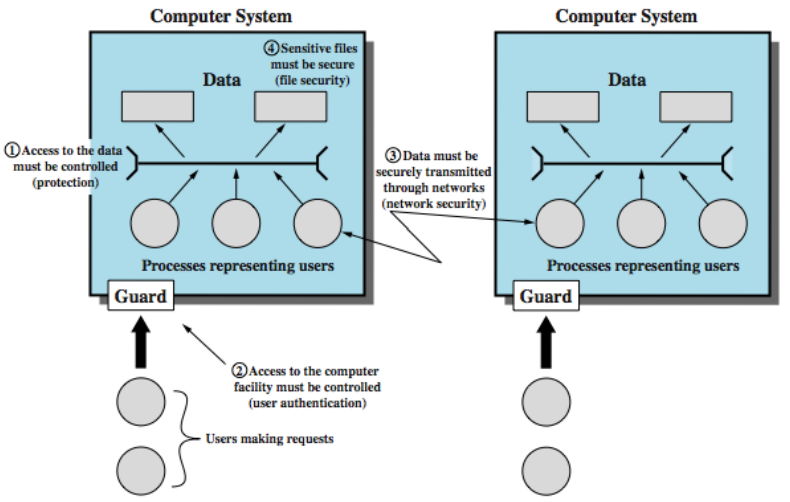
\includegraphics[width=0.7\linewidth]{securityScope}
  \end{center}
\end{frame}

\begin{frame}{Network Security Attacks}
  \begin{itemize}
    \item  classify as passive or active 
    \item  passive attacks are eavesdropping 
      \begin{itemize}
      \item release of message contents 
      \item traffic analysis 
      \item are hard to detect so aim to prevent 
    \end{itemize}
    \item active attacks modify/fake data 
      \begin{itemize}
      \item masquerade 
      \item replay 
      \item modification 
      \item denial of service 
      \item hard to prevent so aim to detect 
    \end{itemize}
    \item  \todo{Networking Security class next term}
    \end{itemize}
\end{frame}

\begin{frame}{Security Functional Requirements}
  \begin{itemize}
  \item technical measures: 
    \begin{itemize}
      \item access control; identification \& authentication; system \& 
      communication protection; system \& information integrity 
    \end{itemize}
  \item management controls and procedures 
    \begin{itemize}
      \item awareness \& training; audit \& accountability; certification, 
      accreditation, \& security assessments; contingency planning; 
      maintenance; physical \& environmental protection; planning; 
      personnel security; risk assessment; systems \& services 
      acquisition 
    \end{itemize}
  \item overlapping technical and management: 
    \begin{itemize}
      \item configuration management; incident response; media protection
    \end{itemize}
  \end{itemize}
\end{frame}

\begin{frame}{X.800 Security Architecture}
  \begin{itemize}
    \item X.800, Security Architecture for OSI 
    \item systematic way of defining requirements for 
    security and characterizing approaches to 
    satisfying them 
    \item defines: 
      \begin{itemize}
        \item security attacks - compromise security 
        \item security mechanism - act to detect, prevent, 
        recover from attack 
        \item security service - counter security attacks 
      \end{itemize}
  \end{itemize}
\end{frame}

\end{document}




%%% Local Variables: 
%%% mode: latex
%%% TeX-master: t
%%% End: 
